\documentclass{standalone}
\usepackage[svgnames]{xcolor}
\usepackage{pgfplots}
\begin{document}
  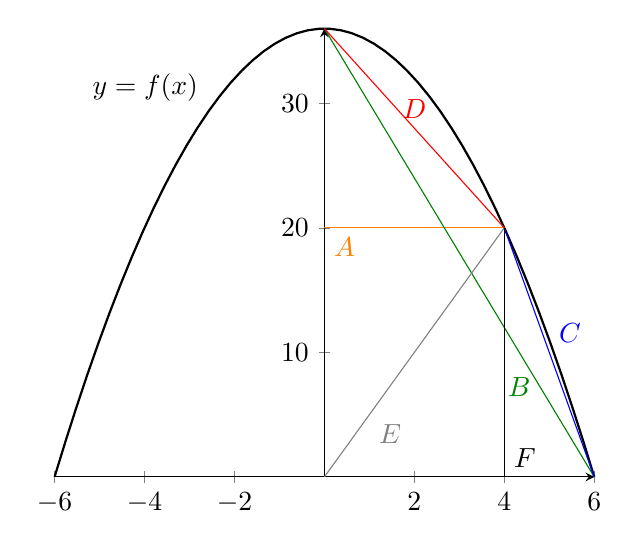
\begin{tikzpicture}
     \begin{axis}[
       axis lines = middle,
       clip=false,
     ]
     \addplot[thick, domain=-6:6, samples=50]{36 - x^2} node[above left, pos=0.4]{\(y=f(x)\)};
     \addplot[color=orange] coordinates {(0,20) (4,20)} node[below right, pos=0]{\(A\)};
     \addplot[color=Green] coordinates {(0,36) (6,0)} node[left, pos=0.8]{\(B\)};
     \addplot[color=blue] coordinates {(4,20) (6,0)} node[above right, pos=0.5]{\(C\)};
     \addplot[color=red] coordinates {(0,36) (4,20)} node[above, pos=0.5]{\(D\)};
     \addplot[color=gray] coordinates {(0,0) (4,20)} node[below right, pos=0.25]{\(E\)};
     \addplot[color=black] coordinates {(4,0) (4,20)} node[above right, pos=0]{\(F\)};
     \end{axis}
  \end{tikzpicture}

\end{document}
